\documentclass{article}

\usepackage[left = 2cm, right = 2cm]{geometry}
\usepackage{graphicx}
\title{Stretching analysis}

\begin{document}

\maketitle

\iffalse
check_barcode_stretching.m
\fi

In this document we discuss stretching factor analysis

We have $N$ theories, $M$ barcodes, $K$ stretch factors. For each stretch factor, we compute $m_i-w+1$ scores (barcodes have lengths $m_i$, $w$ is sliding-window width for the matrix profile method).

\iffalse
We take
numRows = 1;
numKymos = 2;
numTheories = 1;
sets.lengthN = repmat(10000,1,numTheories);
sets.outFold = 'test/';
sets.strF = 2;
sets.pccScore = 0.9;
sets.lambda = 1000;
\fi

Example barcode
\begin{figure}
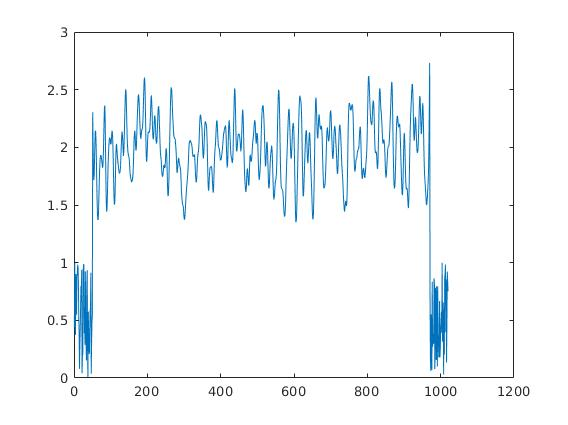
\includegraphics[width=0.6\textwidth]{kymo1.jpg}
\caption{Example barcode (kymograph)}
\end{figure}

Example positions
\begin{figure}
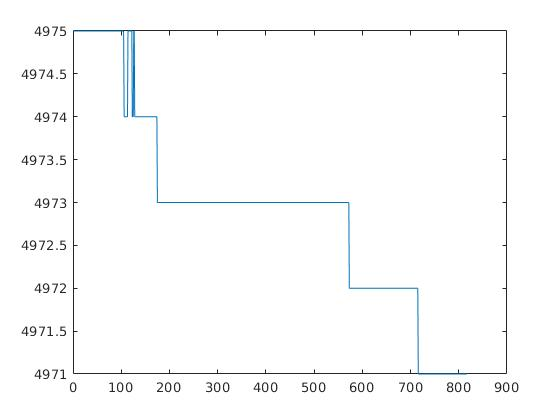
\includegraphics[width=0.6\textwidth]{pos1.jpg}
\caption{Example position values}
\end{figure}

In this example we see that the stretching was a little too big (downward trend in the fitting data) (if the barcode was differently oriented, still would look the same, since the first position is important).

\begin{figure}
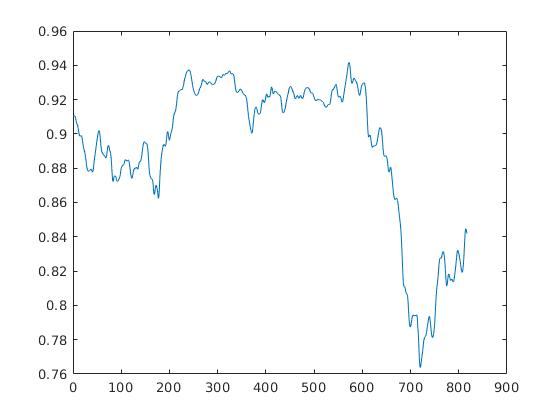
\includegraphics[width=0.6\textwidth]{maxcoef.jpg}
\caption{Correlation coefficients}
\end{figure}


\begin{thebibliography}{10}
\bibitem Marie, Rodolphe, et al. "Single-molecule DNA-mapping and whole-genome sequencing of individual cells." Proceedings of the National Academy of Sciences 115.44 (2018): 11192-11197.
\end{thebibliography}

\end{document}